\chapter{Prototype haute performance}
\label{chap:protoHP}

Dans le cadre d'application comme celui de la réalité augmentée spatiale où les interactions jouent un rôle majeure dans l'expérience de l'utilisateur la réactivité, la fluidité de l'expérience et la latence générale du système sont des points cruciaux qu'il est impossible de négliger. Pour pouvoir atteindre ces objectifs et pouvoir pousser les applications encore plus loin aussi bien dans l'interaction, dans le rendu ou dans le contenu, sans avoir besoin d'une puissance de calcul dépassant l'entendement, une optimisation aussi bien logicielle, matérielle ou architecturale est nécessaire. Cette optimisation a fait l'objet d'une grande partie de mon stage qui m'a amener à développer un prototype dit "haute performance" des outils que propose \texttt{RealityTech}. L'optimisation logicielle a été porté sur l'amélioration des performances des algorithmes de traitement d'image bien connus pour être extrêmement consommateur des ressources. Pour l'optimisation matérielle, la tâche a était un peu différente, nous nous sommes attelé à effectuer des mesures et des calculs sur la puissance théorique du matériel, la latence réel des caméra ou encore la rapidité de l'encodage des flux vidéos pour arriver à établir les performances réelles qu'il nous était possible d'atteindre avec différentes combinaison de matériel. Le développement du prototype s'est achevé avec la création d'une nouvelle architecture logiciel en micro services dans le but de créer un environnement modulaire réactif ou les services peuvent mourir sans mettre en péril tout le système et ainsi améliorer grandement la qualité général des outils fournis.

\section{Amélioration logiciel}
\label{sec:hpsoft}
De nos jour, les optimisations font l'objet de développements ciblés et très spécifique, se concentrant la plupart du temps sur l'amélioration d'un unique point cruciale d'un algorithme ou d'une application. Dans notre cas l'optimisation logiciel a surtout été effectué au niveau des algorithmes de traitement d'images omniprésents et indispensables a la technologie. La réalité augmentée spatiale a besoin du monde réel pour exister c'est pourquoi le matériel dispose de nombreux capteurs (caméras) pour l'analyser et que de nombreux algorithmes de traitement des données captés (images) sont mis en place. Après une rapide analyse du logiciel, il est indéniable que traitement le plus utilisé est la convolution d'une image par un filtre qui possède un nombre incalculable d'application et c'est pourquoi nous avons choisit de concentrer nos efforts sur l'optimisation de ce dernier.

\subsection{Convolution - Théorie}
\begin{quotation}
\textit{En mathématiques, le produit de convolution est un opérateur bilinéaire et un produit commutatif, généralement noté $∗$, qui, à deux fonctions f et g sur un même domaine infini, fait correspondre une autre fonction $f * g$ sur ce domaine, qui en tout point de celui-ci est égale à l'intégrale sur l'entièreté du domaine (ou la somme si celui-ci est discret) d'une des deux fonctions autour de ce point, pondérée par l'autre fonction autour de l'origine — les deux fonctions étant parcourues en sens contraire l'une de l'autre (nécessaire pour garantir la commutativité).\footnote{Source: \href{https://fr.wikipedia.org/wiki/Produit_de_convolution}{Produit de convolution - Wikipedia}}}
\end{quotation}

Dans le cadre du traitement d'image, le produit de convolution représente une technique de filtrage d'image visant à accentuer ou atténuer certaines caractéristiques ce celle ci comme la netteté, le flou ou les zones de fort gradient (les contours) par exemple (fig ~\ref{fig:conv:filter}). Étant donné que nous travaillons avec des images définit par un nombre fini de pixels, la convolution d'une image est réalisée dans le domaine discret où $f$ et $g$ dans la définition mathématique représentent respectivement une image et le filtre qu'on souhaite lui appliquer. Le résultat de cette convolution est une nouvelle image.

On appel filtre, ou noyau de convolution, une image (ou une matrice) généralement de petite taille définit en amont qui va être utilisée pour calculer la nouvelle valeur de chacun des pixels de l'image résultat. C'est la définition de ce dernier qui va décider du traitement appliquer à l'image. 

Le calcul de la valeur d'un pixel dans l'image résultat se fait de la manière suivante : Le voisinage autour du pixel dont on souhaite calculé la valeur est pondéré par le filtre de convolution que l'on aura préalablement centré sur ce pixel. La nouvelle valeur du pixel représente la somme de toutes les valeurs précédemment calculées (voir algorithme ~\ref{algo:pseudo:cpu:conv}).

Sur la figure ~\ref{fig:conv:image} on souhaite calculer la nouvelle valeur du pixel positionné en 3,3 dans l'image d'origine (I). On sélectionne donc un voisinage de même taille que le filtre (K) centré sur ce pixel dont chaque élément va être multiplié par la valeur du filtre pour calculée la valeur du pixel 3,3 dans la nouvelle image soit: 
\begin{center}
$I_{3,3} * K = 88 * 1/9 + 21 * 1/9 + 25 * 1/2 + 68 * 1/9 + 14 * 1/9 + 15 * 1/9 + 35 * 1/9 + 52 * 1/9 + 10 * 1/9 = 36$
\end{center}.


\begin{figure}[H]
\centering
	\subfloat[Image originale]{
      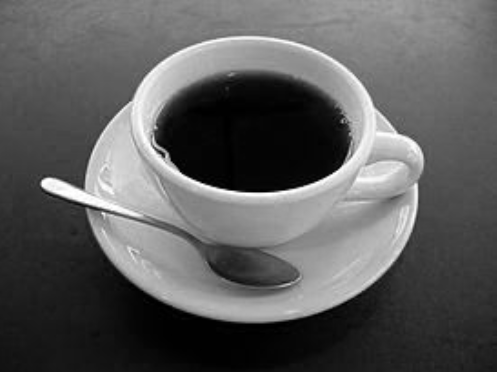
\includegraphics[width=0.33\textwidth]{images/coffee-identity}
      \label{sub:conv:filter:original}
      }
     \subfloat[Filtre contour]{
      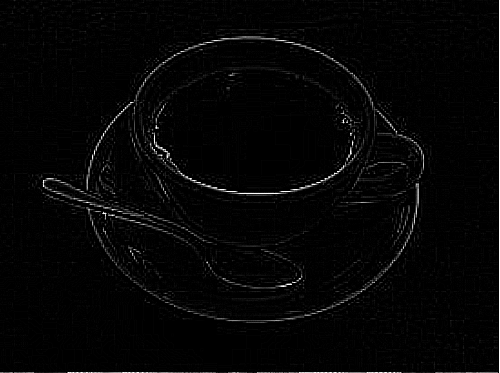
\includegraphics[width=0.33\textwidth]{images/coffee-outline}
      \label{sub:conv:filter:outline}
      }
      \\
      	\subfloat[Filtre de netteté]{
      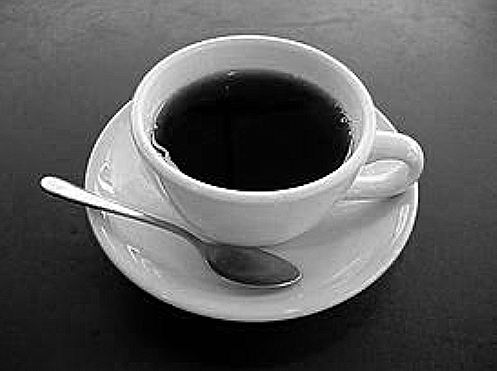
\includegraphics[width=0.33\textwidth]{images/coffee-sharpen}
      \label{sub:conv:filter:sharpen}
      }
     \subfloat[Filtre relief]{
      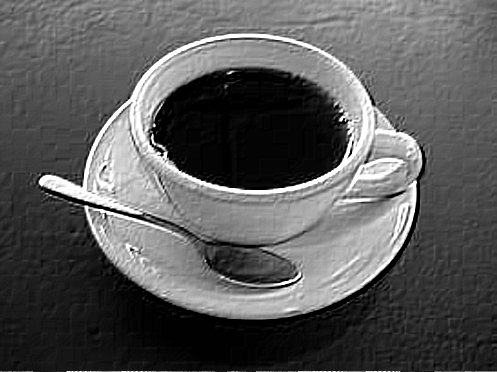
\includegraphics[width=0.33\textwidth]{images/coffee-emboss}
      \label{sub:conv:filter:emboss}
      }
\caption{Différentes filtres de convolution appliquée à une image.}
\label{fig:conv:filter}
\end{figure}

\begin{figure}[H]
\centering
\begin{tikzpicture}
	\matrix (mtr) [matrix of nodes,row sep=-\pgflinewidth, nodes={draw,  minimum size=5.7mm, anchor=center}]
	{
		12 & 46  & 05 & 94 & 25 & 00 & 87\\
		05 & 13  & 01 & 20 & 25 & 00 & 37\\
		72 & 25  & |[fill=red!30]| 88 & |[fill=red!30]| 21 & |[fill=red!30]| 25 & 00 & 99\\
		21 & 74  & |[fill=red!30]| 68 & |[fill=red!30]| 14 & |[fill=red!30]| 15 & 00 & 61\\
		48 & 97  & |[fill=red!30]| 35 & |[fill=red!30]| 52 & |[fill=red!30]| 10 & 00 & 42\\
		11 & 29  & 57 & 00 & 75 & 00 & 12\\
		17 & 01  & 78 & 00 & 50 & 00 & 12\\
		16 & 54  & 00 & 00 & 25 & 00 & 11\\
	};

	\draw[very thick, red] (mtr-3-3.north west) rectangle (mtr-5-5.south east);

	\node [below= of mtr-8-4.south] (lm) {$\bf I$};
	\node[right = 0.2em of mtr] (str) {$* \frac{1}{9}$};

	\matrix (K) [right=0.2em of str,matrix of nodes,row sep=-\pgflinewidth, nodes={draw, fill=blue!30,  minimum size=5.7mm, anchor=center}]
	{
		1 & 1 & 1 \\
		1 & 1 & 1 \\
		1 & 1 & 1 \\
	};
	\node [below = of K-3-2.south] (lk) {$\bf K$};

	\node [right = 0.2em of K] (eq) {$=$};

	\matrix (ret) [right=0.2em of eq,matrix of nodes,row sep=-\pgflinewidth, nodes={draw, minimum size=5.7mm, anchor=center}, nodes in empty cells]
	{
		 &   &  &  &  &  & \\
		 &   &  &  &  &  & \\
		 &   &  &  &  &  & \\
		 &   &  & |[fill=green!30]| 36 &  &  & \\
		 &   &  &  &  &  & \\
		 &   &  &  &  &  & \\
		 &   &  &  &  &  & \\
		 &   &  &  &  &  & \\
	};
	\node [below = of ret-8-4.south] (lim) {${\bf I_{i,j}} * {\bf K}$};

	\draw[very thick, green] (ret-4-4.north west) rectangle (ret-4-4.south east);

	\draw[densely dotted, blue, thick] (mtr-3-3.north west) -- (K-1-1.north west);
	\draw[densely dotted, blue, thick] (mtr-5-3.south west) -- (K-3-1.south west);
	\draw[densely dotted, blue, thick] (mtr-3-5.north east) -- (K-1-3.north east);
	\draw[densely dotted, blue, thick] (mtr-5-5.south east) -- (K-3-3.south east);

	\draw[densely dotted, green, thick] (ret-4-4.north west) -- (K-1-1.north west);
	\draw[densely dotted, green, thick] (ret-4-4.south west) -- (K-3-1.south west);
	\draw[densely dotted, green, thick] (ret-4-4.north east) -- (K-1-3.north east);
	\draw[densely dotted, green, thick] (ret-4-4.south east) -- (K-3-3.south east);

	\draw[very thick, blue] (K-1-1.north west) rectangle (K-3-3.south east);

	\node[anchor=south east, inner sep=0.01em, blue] at (mtr-3-3.south east) (xx) {\scalebox{.5}{$\times 1$}};
	\node[anchor=south east, inner sep=0.01em, blue] at (mtr-3-4.south east) (xx) {\scalebox{.5}{$\times 1$}};
	\node[anchor=south east, inner sep=0.01em, blue] at (mtr-3-5.south east) (xx) {\scalebox{.5}{$\times 1$}};
	\node[anchor=south east, inner sep=0.01em, blue] at (mtr-4-3.south east) (xx) {\scalebox{.5}{$\times 1$}};
	\node[anchor=south east, inner sep=0.01em, blue] at (mtr-4-4.south east) (xx) {\scalebox{.5}{$\times 1$}};
	\node[anchor=south east, inner sep=0.01em, blue] at (mtr-4-5.south east) (xx) {\scalebox{.5}{$\times 1$}};
	\node[anchor=south east, inner sep=0.01em, blue] at (mtr-5-3.south east) (xx) {\scalebox{.5}{$\times 1$}};
	\node[anchor=south east, inner sep=0.01em, blue] at (mtr-5-4.south east) (xx) {\scalebox{.5}{$\times 1$}};
	\node[anchor=south east, inner sep=0.01em, blue] at (mtr-5-5.south east) (xx) {\scalebox{.5}{$\times 1$}};
\end{tikzpicture}
\caption{Convolution d'une matrice (image) (I) par un filtre (K)}
\label{fig:conv:image}
\end{figure}

\begin{algorithm}[H]
	\caption{Convolution d'image image par un filtre}
	\begin{algorithmic}
		\Procedure{Convolution}{I, K, Iw, Ih, Ks}\Comment{I: image, K: filtre}
		\State $I_{conv} \gets I$
		\State $Khs \gets floor(Ks \div 2)$
		\State $x \gets 0, y \gets 0$
		\State $sum \gets 0$
		\For{$x \leq Iw ; ++x$}
			\For{$y \leq Ih ; ++y$}\Comment{Pour tous les pixels $x,y$}
				\For{$i \leq Ks ; ++j$}
					\For{$j \leq Ks ; ++j$}\Comment{Pour chaque éléments dans une fenêtre de taille $Ks$}
					\State ${pos_x \gets x + i - Ksh}$ \Comment{pos = pos + position dans le voisinage}
					\State ${pos_y \gets y + j - Ksh}$ \Comment{pos = pos + position dans le voisinage}
					\If{$outOf(I, pos_x, pos_y)$} \Comment{Vérifie que les positions sont dans l'image (bords)}
						\State $continue$
					\EndIf
					\State $sum \gets sum + I_{pos_x, pos_y} * K{i, j}$ \Comment{Somme du voisinage par le filtre}
					\State $maskSum \gets maskSum + K{i, j}$
					\EndFor
				\EndFor
				\State $I_{conv}{x, y} \gets sum \div maskSum$ \Comment{Valeur final = somme normalisée}
			\EndFor
		\EndFor
		\State \Return $I_{conv}$ \Comment{Retourne la nouvelle image}
		\EndProcedure
	\end{algorithmic}
	\label{algo:pseudo:cpu:conv}
\end{algorithm}

Comme on peut s'en rendre compte dans le pseudo code proposé (algo ~\ref{algo:pseudo:cpu:conv}), l'image résultat est une nouvelle image, indépendante de l'image d'origine dont chaque pixel est calculé indépendamment de ces voisins dans cette nouvelle image. Cela signifie que n'importe quel pixel peut être calculé dans n'importe quel ordre. C'est précisément à cette propriété que nous allons nous intéresser car en théorie, avec une puissance de calcul suffisante il est possible de calculer en même temps tous les pixels de l'image résultat. Cet algorithme possède donc un très fort potentiel d'optimisation car il est très largement parallélisable.

%C'est cette propriété qui va nous intéressé car cela signifie qu'il est possible de calculer chaque pixel de l'image résultat dans n'importe quel ordre et qu'avec des moyens de calculs suffisant il est possible de calculer tous les pixels de l'image résultat en une seule fois. On dit d'une telle fonction qu'elle est parallélisable. Ce fort potentiel de parallélisation fait de ce traitement une cible de choix pour l'optimisation et donc le calcul sur carte graphique (section ~\ref{chap:notions} - Calcul haute performance).

\subsection{Convolution - Optimisation}
L'optimisation de cet algorithme peut se faire de deux façon bien distinctes. La première se fait en utilisant la puissance de la carte graphique de l'ordinateur pour effectuer énormément de calculs en même temps. C'est l'optimisation sur carte graphique dont nous avons évoqué le principe chapitre ~\ref{chap:notions}. La seconde méthode d'optimisation consiste à légèrement changer l'algorithme de convolution: la convolution est séparé en deux filtres distincts\cite{podlozhnyuk2007image}, un horizontal et un vertical qui sont successivement appliqués à l'image origine (fig ~\ref{fig:conv:separable}). Ainsi la complexité d'appliquer une convolution de taille $MxM$ a une image de taille $NxN$ est réduit de $O(N^2M^2)$ a $O(N^2M)$.

\begin{figure}[H]
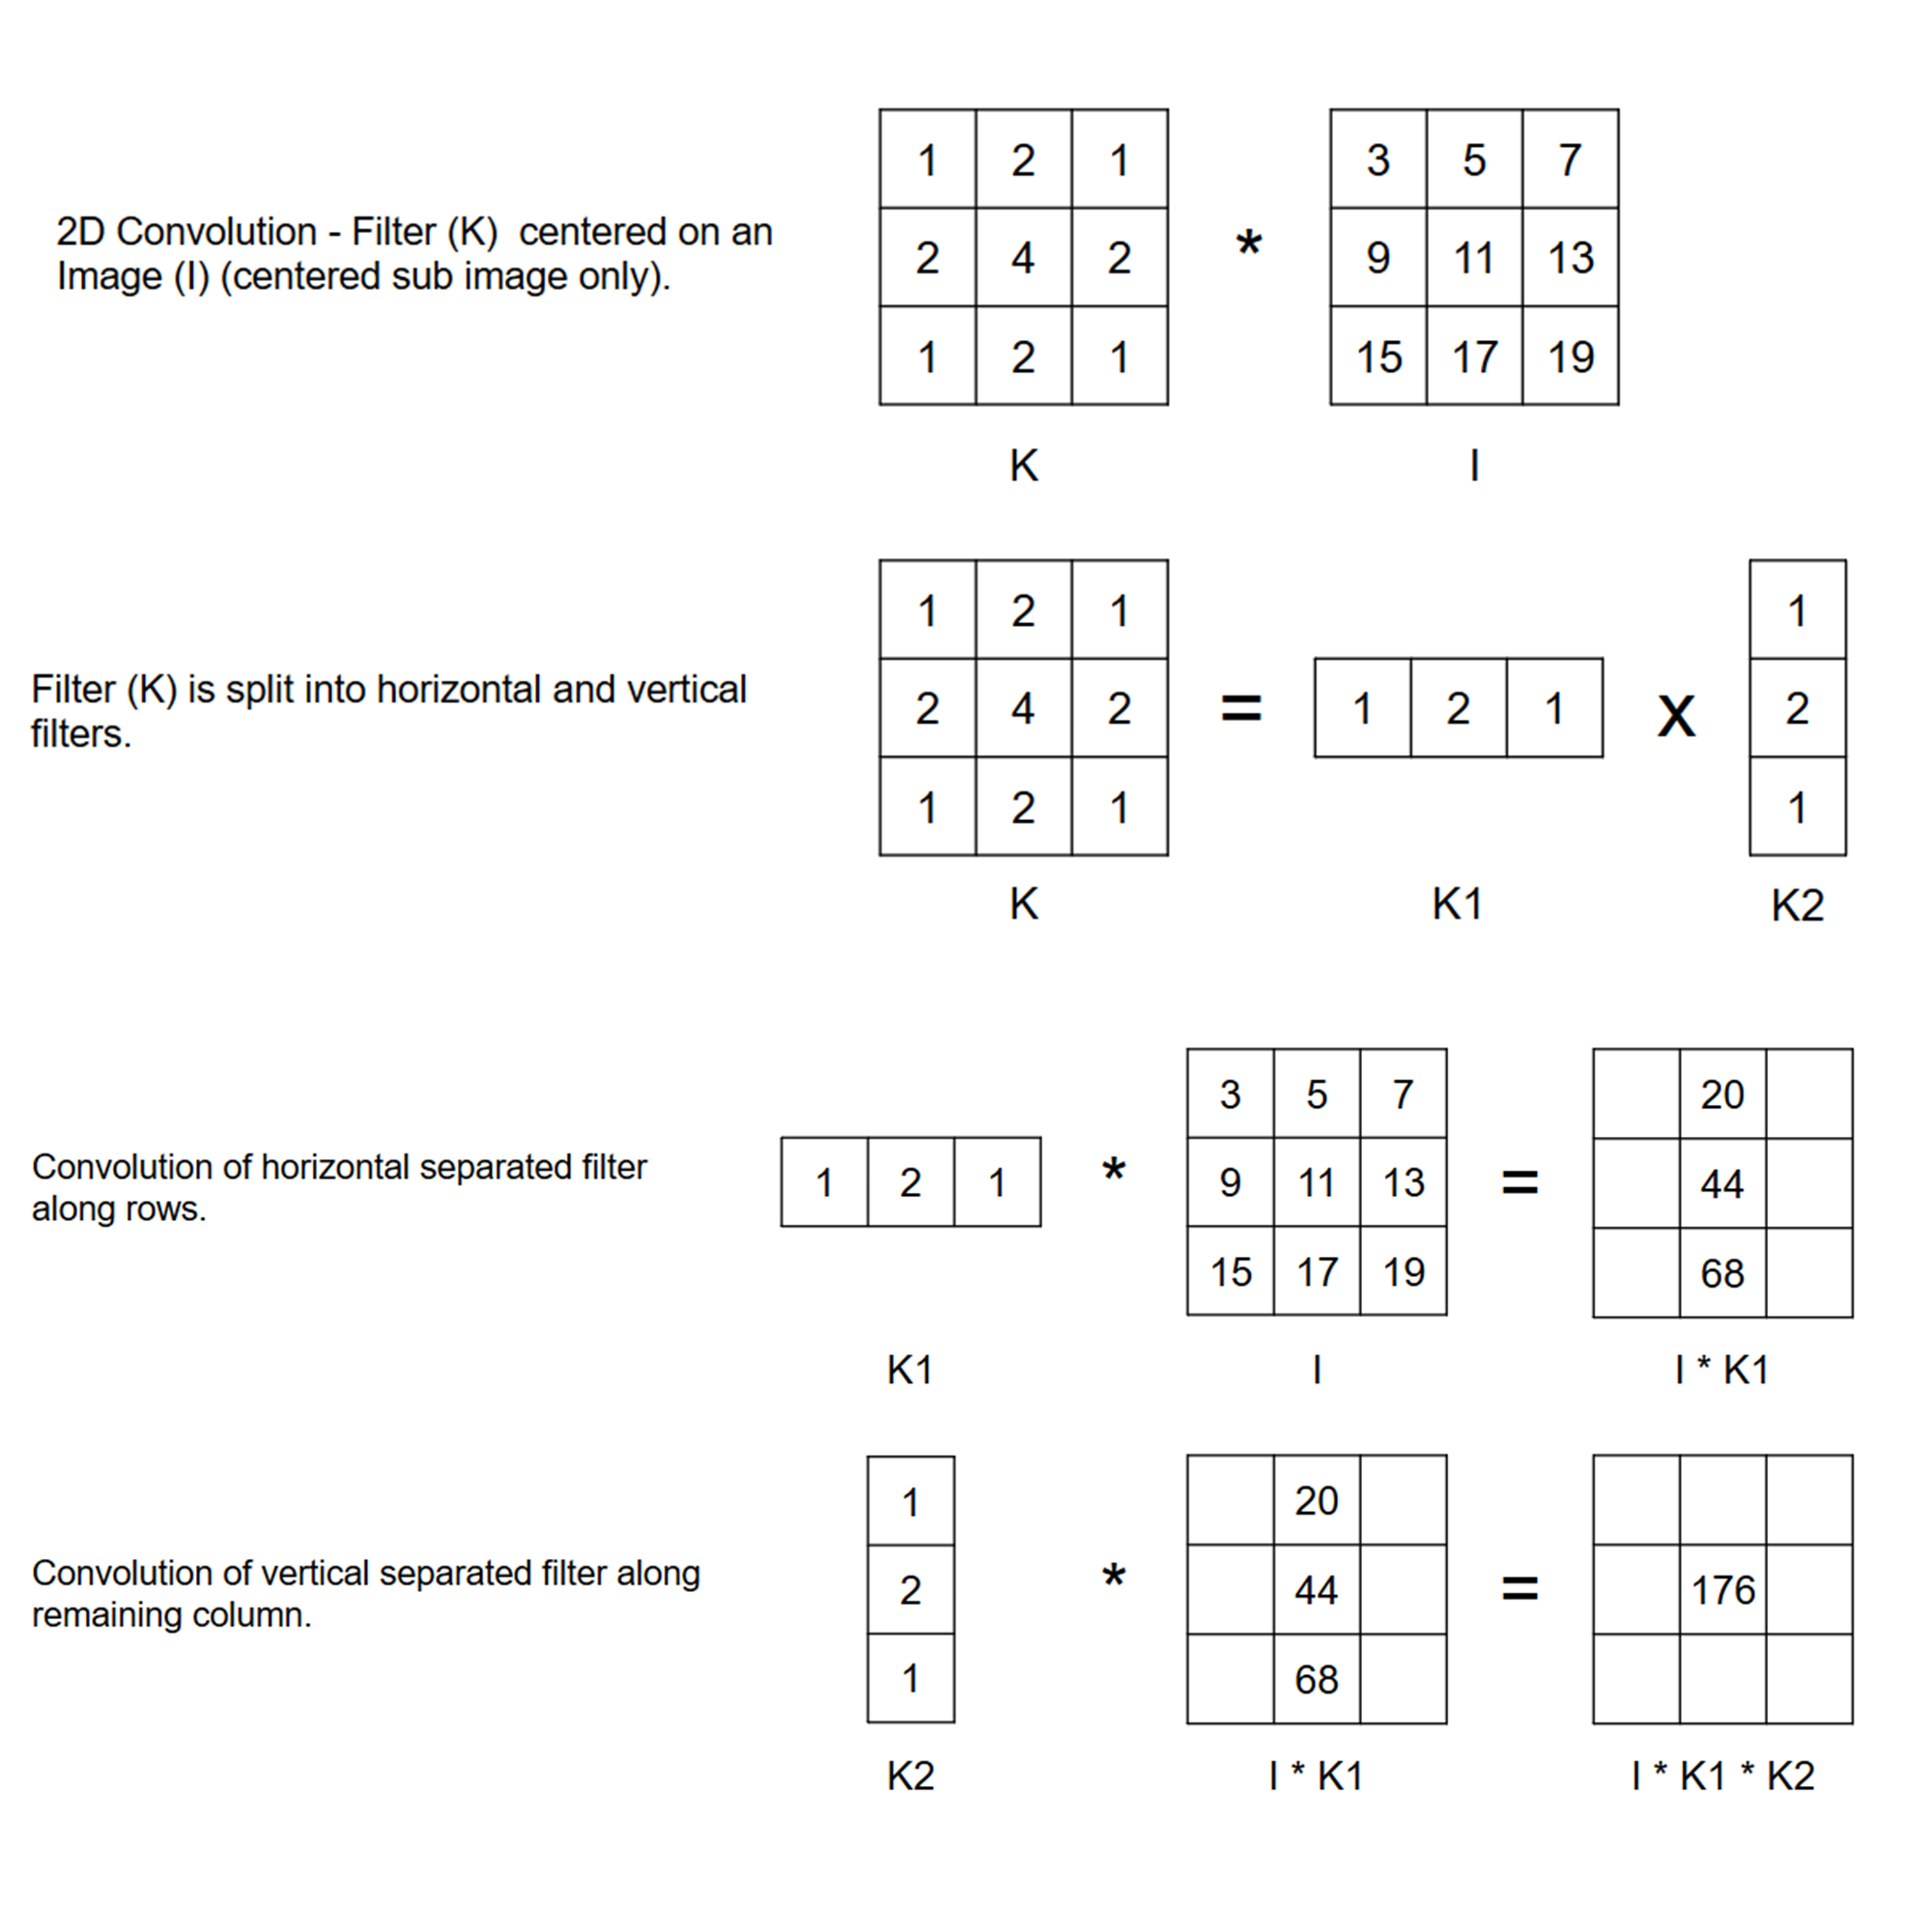
\includegraphics[width=\linewidth]{images/separableconv}
\caption{Exemple d'un filtre de convolution appliqué successivement horizontalement puis verticalement}
\label{fig:conv:separable}
\end{figure}

Nous avons choisit de n'effectuer que l'optimisation sur carte graphique car la deuxième méthode comporte un gros coût en complexité et en temps de développement que nous n'avons pas juger nécessaire d'inclure dans cette première version. De plus il n'est pas toujours possible de séparé un filtre $K$ en 2 sous filtres $K1, K2$ tel que $K = K1 \times K2$.

Pour pouvoir développer la dite optimisation, il a fallut utiliser un langage de programmation sur carte graphique. De nos jours, il en existe plusieurs et ils possèdent tous leurs spécificités cependant pendant la phase de recherche, 3 langages (ou sous langages) se sont démarqués : OpenCL\cite{opencl}, OpenGL ES\cite{opengles} et CUDA\cite{cuda}. Nous avons donc choisit d'implémenter 3 version de l'algorithme de convolution naïf (non séparé) utilisant chaque de ces langages et d'en évaluer les performances.

\paragraph{OpenCL} OpenCL ou \emph{Open Computing Language} est un langage de programmation basé sur le C créé par \texttt{Khronos Group} en 2009.
Un programme OpenCL s'écrit en deux partie:
La partie \textbf{code hôte} et la partie \textbf{noyau} ou \textbf{code périphérique} qui représentent respectivement la partie application se chargeant d'orchestrer les différentes et tâches, la gestion mémoire, la gestion des périphériques s'exécutant sur l'hôte et la partie calcul permettant de compléter les dites tâches s'exécutant sur les périphériques. La partie hôte est écrite en C tandis que la partie noyau est écrit en OpenCL-C.
Il faut donc aussi différencier hôte et périphérique (fig ~\ref{fig:opencl}). Dans notre cas d'utilisation l'hôte représente le processeur et permet de transmettre les données au périphérique qui dans notre cas correspond à une ou plusieurs cartes graphiques.

\begin{figure}[H]
\centering
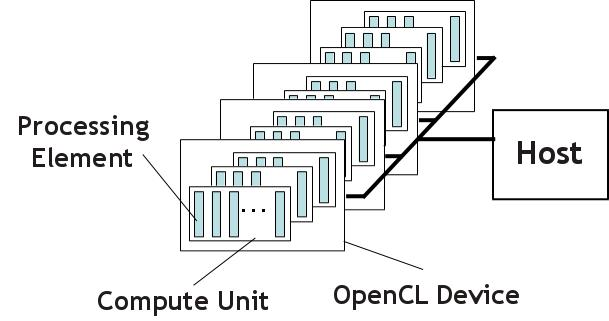
\includegraphics[width=0.5\linewidth]{images/opencl}
\caption{Schéma OpenCL - Hôte et périphériques\protect\footnotemark}
\label{fig:opencl}
\end{figure}

\footnotetext{Source: \href{https://www.anandtech.com/show/7334/a-look-at-alteras-opencl-sdk-for-fpgas/2}{https://www.anandtech.com/show/7334/a-look-at-alteras-opencl-sdk-for-fpgas/2}}

Nous nous sommes intéressé a OpenCL car il est compatible avec la plupart des systèmes et des architectures aujourd'hui présents sur le marché sans aucune modification de code nécessaire. Cet avantage est aussi l'un de ses plus gros inconvénients car il ne permet pas d'exploiter au mieux chaque architecture comme peut le faire CUDA avec NVIDIA, et les performances de ce dernier ne sont donc pas équivalentes sur chaque architecture. %Parler dans le bilan Le coût de développement de traitement en OpenCL tout aussi lour

\paragraph{OpenGL (ES)} 
OpenGL est une interface de programmation multi plateforme et multi langage permettant faire le rendu de scène 2D/3D. En tant qu'interface il est possible de l'implémenter de façon logiciel mais elle a été conçu pour être implémenté de manière matérielle avec de profiter au mieux des accélérations matérielles disponibles. Ainsi c'est grâce à ces implémentation qu'OpenGL fournit un \emph{pipeline} programmable de rendu ultra performant. C'est via ce pipeline programmable et plus spécifiquement via le code hôte et les shaders qu'il est possible de transmettre des instructions et des données à la carte graphique (fig ~\ref{fig:opengl:pipeline})

\begin{figure}[H]
\centering
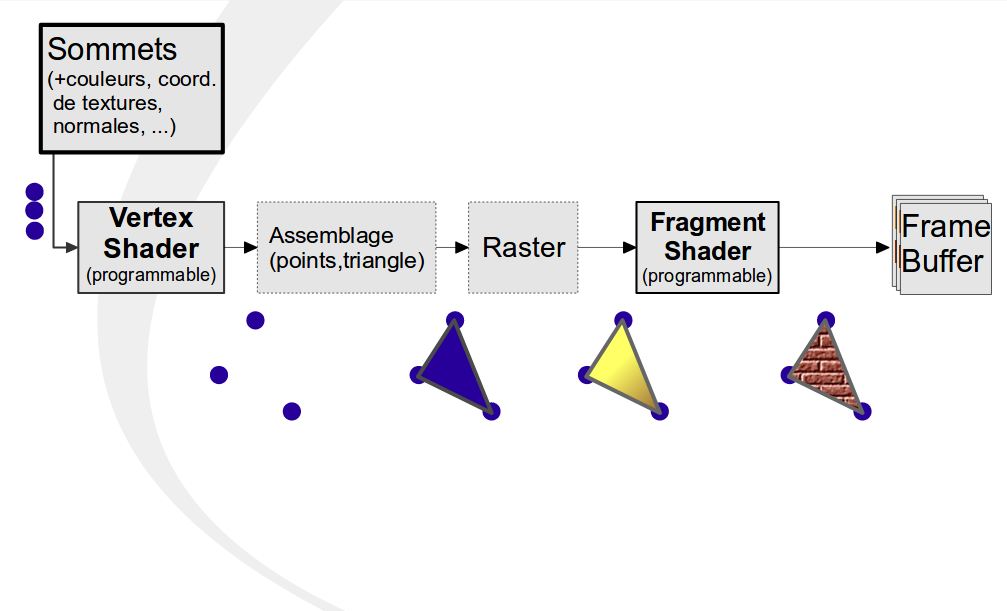
\includegraphics[width=\linewidth]{images/opengl-pipeline}
\caption{Pipeline de rendu - OpenGL\protect\footnotemark}
\end{figure}

\footnotetext{Source: \href{http://www.labri.fr/perso/pbenard/teaching/mondes3d/slides/Cours_Monde3D_2017_04-IntroGL.pdf}{Cours M1 Informatique - Mondes 3D - Pierre Benard}}

Le pipeline OpenGL reçoit en entrée:
\begin{itemize}
\item Des informations sur la géométrie de la scène.
\item Des paramètres nécessaire pour effectuer le rendu de la scène. Point de vue de la caméra, lumières, textures, matériaux.
\end{itemize}
et donne en sortie une image de la scène.

Pour pouvoir utiliser ce pipeline dans le but d'opérer des traitements sur des images 2D, il est nécessaire d'en détourner l'utilisation. Sans géométrie a fournir au vertex shader, le pipeline de rendu ne se déclenche pas. L'idée pour passer outre est de créer un bout de géométrie recouvrant l'écran, le plus souvent un quad, afin d'activer le pipeline. Une fois le pipeline activité, le vertex shader est programmé pour ne rien faire  et ainsi les étapes d'assemblage et de rastérisation sont très rapidement passé pour arriver à l'étape du rendu par fragment. C'est dans ce shader que se compose l'image de sortie du rendu et c'est ici que nous avons access à tout les pixels de l'image. Le calcul de la convolution se fait donc pour chaque pixel grâce au code présent dans le fragment shader. Une fois le traitement par fragment effectué, l'image résultat est stockée dans le \emph{Frame Buffer Object ou FBO} et peut être récupéré depuis l'hôte.

L'avantage de cette technique est que comme OpenCL, OpenGL (ESà est largement compatible sur toutes les plateforme et très largement utilisé. Cependant, contrairement à OpenCL, les performances d'OpenGL ne dépendent que du matériel et ne varieront pas ou que très peu d'un système à un autre.

\paragraph{CUDA} CUDA, contrairement a OpenCL et OpenGL n'est pas seulement un langage de programmation mais bel et bien une architecture de traitement parallèle développée par NVIDIA dont l'unique but est d'exploiter la carte graphique a son maximum pour offrir une énorme puissance de calcul au système l'utilisant. Pour ce qui est de la partie programmation, NVIDIA fournis une API permettant d'utiliser cette architecture, CUDA C, et qui fonctionne de façon similaire a OpenCL avec du code hôte et du code périphérique qui seront les noyaux CUDA à exécuter sur la carte graphique. La ou CUDA se démarque c'est dans le modèle qu'il propose, les tâches ou \emph{threads} sont regroupés en blocs ou \emph{blocks} à l'intérieur desquels la mémoire est partagée et ou chaque bloc s'exécute sur exactement une unité de calcul (fig. ~\ref{fig:cuda:archi}), la mémoire est unifiée (fig ~\ref{fig:cuda:unifiedmemory}), les CPUs et les GPUs ont accès à la même mémoire sans besoin des copies ce qui permet réduire énormément les temps de transfert des données.

\begin{figure}[H]
\centering
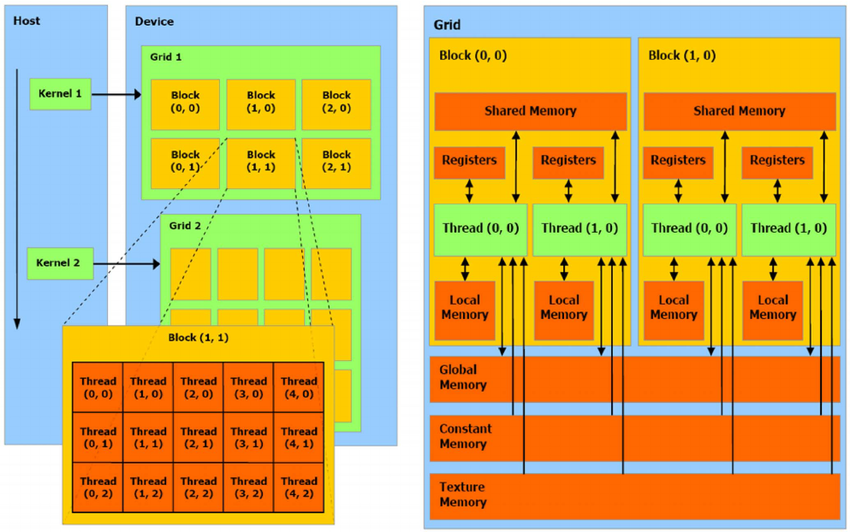
\includegraphics[width=0.9\linewidth]{images/cuda-archi}
\caption{Représentation schématique de l'architecture CUDA\protect\footnotemark}
\label{fig:cuda:archi}
\end{figure}
\footnotetext{Source: \href{http://programming4.us/enterprise/18672.aspx}{NVIDIA CUDA - Unified Device Architecture}}

\begin{figure}[H]
\centering
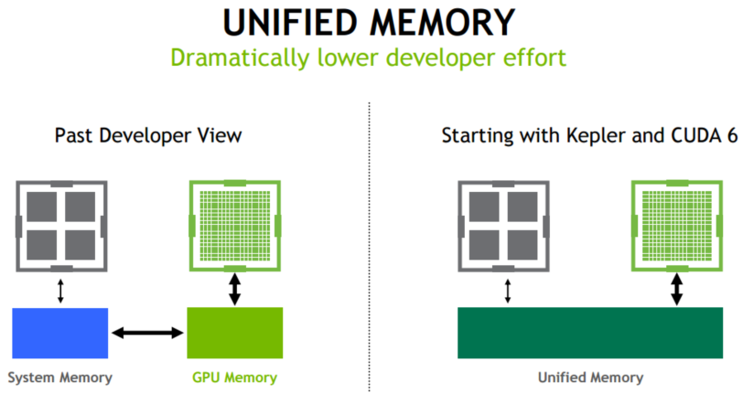
\includegraphics[width=0.65\linewidth]{images/cuda-unified-memory}
\caption{Mémoire séparé vs mémoire unifiée\protect\footnotemark}
\label{fig:cuda:unifiedmemory}
\end{figure}
\footnotetext{Source: \href{https://devblogs.nvidia.com/unified-memory-cuda-beginners/}{NVIDIA CUDA - Unified Memory for beginners}}

CUDA étant une architecture matériel seul les cartes graphique NVIDIA récentes en sont équipé ce qui contrairement aux deux autres ne le rend absolument pas multiplateforme.

\subsection{Tests de performances}
\label{sub:conv:bench}
Afin de comparer les différentes solutions nous avons réaliser des tests de performances du même algorithme de convolution que nous avons implémenté dans les différents langages cités et sur différentes machines avec des configuration bien différentes. Le but de ces tests était dans un premier temps d'observer l'impacte de l'optimisation et dans un second temps d'orienter le choix d'ordinateur à inclure dans le système de RealityTech en se basant sur les résultats obtenues en fonction des différentes plateforme.

A noter que l'algorithme de convolution implémenté est la version non séparé ou le filtre de convolution est considéré comme une matrice.

Dans ce test de performances, nous avons mesurer plusieurs choses:
\begin{itemize}
\item \textbf{Le temps de transfert} des données de l'hôte au périphérique. Cette mesure est importante car elle permet d'évaluer l'impact de la mémoire unifiée CUDA par rapport aux autres méthodes ne possédant pas cette fonctionnalité.
\item \textbf{Le temps de calcul} brut de la convolution de l'image. Afin d'évaluer les performances brut de l'algorithme par langages, nous avons mesurer les temps de calcul de chacun.
\item \textbf{La "bande passante"} du traitement entier, comprenant transfert calcul et re transfert. Cette mesure donne une bonne idée de la rapidité des algorithme car elle exprime le nombre de méga octet qu'il est possible de traiter en une seconde avec chaque implémentation.
\end{itemize}

\textbf{Note:} Les résultats donnés Tableau ~\ref{fig:conv:benchmark} ont été mesuré sur le kit de développement NVIDIA Tegra Jetson TX2 dont les spécificité sont les suivantes: \texttt{CPU ARM ARM Cortex-A57 (quad-core) @ 2GHz + NVIDIA Denver2 (dual-core) @ 2GHz, GPU 256-core Pascal @ 1300MHz, RAM 8GB 128-bit LPDDR4 @ 1866Mhz |  59.7 GB/s} Nous avons choisit de montrer ici seulement les résultats obtenues sur le kit de developpement NVIDIA car il permet d'observer les performances de CUDA dans un environnement ultra optimisé pour ce dernier cependant vous trouverez Annexe %TODO
les résultats de ces mêmes test sur plusieurs ordinateurs différents.

\begin{table}[H]
\centering
\caption{CUDA 9.0 - Convolution d'une image en niveau de gris par un filtre de taille 5x5 - float 32bits}
\label{fig:conv:benchmark}
\resizebox{\textwidth}{!}{%
\begin{tabular}{|c|c|c|c|c|c|}
\hline
\textbf{Size} & \textbf{Size (MB)} & \textbf{Compute Time (ms)} & \textbf{Transfer Time (ms)} & \textbf{Total Time (ms)} & \textbf{Bandwidth (MB/s)} \\ \hline
\cellcolor{green!40}\textbf{128x128} & 0,0655 & 0,0964 & 0,7737 & \cellcolor{green!40}0,8701 & 75,3224 \\ \hline
\cellcolor{green!40}\textbf{256x256} & 0,2621 & 0,2222 & 1,8457 & \cellcolor{green!40}2,0679 & 126,7661 \\ \hline
\cellcolor{green!40}\textbf{512x512} & 1,0486 & 0,8764 & 3,5266 & \cellcolor{green!40}4,4030 & 238,1503 \\ \hline
\cellcolor{green!40}\textbf{1024x1024} & 4,1943 & 3,2107 & 9,1959 & \cellcolor{green!40}12,4066 & 338,0703 \\ \hline
\cellcolor{orange!70}\textbf{2048x2048} & 16,7772 & 12,7048 & 35,0284 & \cellcolor{orange!70}47,7332 & 351,4786 \\ \hline
\cellcolor{red!40}\textbf{4096x4096} & 67,1089 & 51,0330 & 139,0710 & \cellcolor{red!40}190,1040 & 353,0115 \\ \hline
\cellcolor{red!40}\textbf{8192x8192} & 268,4350 & 210,2130 & 553,8050 & \cellcolor{red!40}764,0180 & 351,3464 \\ \hline
\end{tabular}%
}
\end{table}

\begin{table}[H]
\centering
\caption{OpenGL ES 2.0 - Convolution d'une image en niveau de gris par un filtre de taille 5x5 - float 32bits}
\label{fig:bench:opengles}
\resizebox{\textwidth}{!}{%
\begin{tabular}{|c|c|c|c|c|c|}
\hline
\textbf{Size} & \textbf{Size (MB)} & \textbf{Compute Time (ms)} & \textbf{Transfer Time (ms)} & \textbf{Total Time (ms)} & \textbf{Bandwidth (MB/s)} \\ \hline
\cellcolor{green!40}\textbf{128x128} & 0,0655 & 0,1386 & 0,9038 & \cellcolor{green!40}1,0424 & 62,8703 \\ \hline
\cellcolor{green!40}\textbf{256x256} & 0,2621 & 0,0202 & 1,3858 & \cellcolor{green!40}1,4060 & 186,4475 \\ \hline
\cellcolor{green!40}\textbf{512x512} & 1,0486 & 0,0194 & 4,2613 & \cellcolor{green!40}4,2807 & 244,9576 \\ \hline
\cellcolor{green!40}\textbf{1024x1024} & 4,1943 & 0,0212 & 15,6039 & \cellcolor{green!40}15,6251 & 268,4337 \\ \hline
\cellcolor{red!40}\textbf{2048x2048} & 16,7772 & 0,0215 & 60,8093 & \cellcolor{red!40}60,8309 & 275,8008 \\ \hline
\cellcolor{red!40}\textbf{4096x4096} & 67,1089 & 0,0215 & 241,5410 & \cellcolor{red!40}241,5625 & 277,8117 \\ \hline
\cellcolor{red!40}\textbf{8192x8192} & 268,4350 & 0,0267 & 1163,1867 & \cellcolor{red!40}1163,2133 & 230,7702 \\ \hline
\end{tabular}%
}
\end{table}

\begin{table}[H]
\centering
\caption{CPU - Convolution d'une image en niveau de gris par un filtre de taille 5x5 - float 32bits}
\label{fig:bench:cpu}
\resizebox{\textwidth}{!}{%
\begin{tabular}{|c|c|c|c|c|c|}
\hline
\textbf{Size} & \textbf{Size (MB)} & \textbf{Compute Time (ms)} & \textbf{Transfer Time (ms)} & \textbf{Total Time (ms)} & \textbf{Bandwidth (MB/s)} \\ \hline
\cellcolor{green!40}\textbf{128x128} & 0,0655 & 8,3513 & 0,0000 & \cellcolor{green!40}8,3569 & 7,8421 \\ \hline
\cellcolor{green!40}\textbf{256x256} & 0,2621 & 33,8604 & 0,0000 & \cellcolor{green!40}33,8698 & 7,7398 \\ \hline
\cellcolor{red!40}\textbf{512x512} & 1,0486 & 150,1860 & 0,0000 & \cellcolor{red!40}150,2010 & 6,9812 \\ \hline
\cellcolor{red!40}\textbf{1024x1024} & 4,1943 & 721,2130 & 0,0000 & \cellcolor{red!40}721,2310 & 5,8155 \\ \hline
\cellcolor{red!40}\textbf{2048x2048} & 16,7772 & 3196,6300 & 0,0000 & \cellcolor{red!40}3196,6500 & 5,2484 \\ \hline
\cellcolor{red!40}\textbf{4096x4096} & 67,1089 & 13130,9000 & 0,0000 & \cellcolor{red!40}13130,9000 & 5,1108 \\ \hline
\cellcolor{red!40}\textbf{8192x8192} & 268,4350 & 53591,6000 & 0,0000 & \cellcolor{red!40}53591,7000 & 5,0089 \\ \hline
\end{tabular}%
}
\end{table}

Comme on peut s'en rendre compte les gains de performances des deux version optimisées de l'algorithme sont non négligeable par rapport a la version CPU naïve (fig ~\ref{fig:bench:cpu}). On observer que les algorithmes s'exécutant sur la carte graphique sont jusqu'à 55 fois plus rapide pour OpenGL ES (fig ~\ref{fig:bench:opengles}) et jusqu'à 70 fois pour la version CUDA (fig~\ref{fig:bench:cuda}). Les cases vertes dans les tableaux indiquent que l'image a pu être traité en pseudo temps réel avec une fréquence de rafraichissement de 25fps qui signifie que pour chaque image à afficher, nous disposons d'un temps de $1/25 * 1000 = 40$ millisecondes pour en faire le rendu.
Au delà de la constat d'optimisation, on peut voir que la version CUDA et la version OpenGL affichent des résultats plutôt similaire, ils sont tout deux capable de traiter en temps réel des images de taille 1024x1024 pixels sans difficulté. On peut cependant noter une différence flagrante entre ces deux versions, en effet, on peut observer le gain apportée par la mémoire unifiée CUDA lorsque l'on compare les temps de transfert avec ceux d'OpenGL. En moyenne les temps de transfert en CUDA sont 2 fois plus rapide que leur équivalent OpenGL ES ce qui a un impact significatif sur les performances car ils correspondent à la majeur partie du temps d'exécution du programme.

% Benchmark + comparaison avec temps GPU

\subsection{Conclusion}
Au vu des résultats obtenues section ~\ref{sub:conv:bench} on peut noter deux choses:
\begin{itemize}
\item L'optimisation de l'algorithme utilisant un filtre de convolution séparé n'aura quasiment aucun impact sur les performances en OpenGL car les temps de calcul sont négligeables par rapport aux temps de transfert ainsi seules les version CUDA et CPU bénéficierons des amélioration qu'il peut potentiellement apporter.
\item CUDA et OpenGL fournissent tout deux des résultats plutôt similaires (avec une potentielle amélioration du côté CUDA) mais n'offre tout les deux pas les mêmes possibilités. Avec CUDA, l'algorithme ne peut tourner que sur des machines supportant l'architecture. Nous avons jugé que le gain apporté par rapport a OpenGL ES, qui lui est totalement, n'était pas suffisant pour contrebalancer ce coût, c'est pourquoi nous avons choisit de continuer à utiliser et développer la version OpenGL ES.
\end{itemize}

\newpage
\section{Amélioration matérielle}
Comme évoqué dans l'introduction, le deuxième axe d'amélioration de la technologie de RealityTech se base sur l'aspect purement matériel du système qu'elle propose.
Dans cette partie, nous avons essayé d'observer et de mesurer la "puissance" du matériel utilisé afin de déterminer les parties cruciale a améliorer.

En premier lieu, nous nous sommes intéressé à mesurer la latence des dispositifs d'acquisition. 
La latence est définit comme le temps écoulé entre l'acquisition et l'affichage d'une information. 
Nous nous sommes donc procuré de nombreuses caméras différentes dont nous avons mesurer la latences sur plusieurs ordinateur. Certains ordinnateurs possèdait des capacités d'encodage vidéo matériel (comme sur le NVIDIA Jetson TX2 obtenue pour l'occasion qui possède un module MSENC, un encodeur matériel\footnote{\href{https://www.nvidia.fr/autonomous-machines/embedded-systems-dev-kits-modules/}{NVIDIA Jetson TX2 - Charactéristiques des modules}}) ce qui nous a permis d'en évaluer l'impacte sur la latence lors de l'obtention du flux vidéo. Mis a part le Jetson TX2 possédant une caméra embarquée, les mesures de la latence ont toutes été effectué en utilisant GStreamer\cite{gstreamer} avec la même commande d'obtention du flux afin d'éviter au maximum les différences de mesure.

Pour mesurer cette latence, nous avons utiliser la méthode dite "Glass to glass" qui est pratiquement la seule méthode actuellement. Pour effectuer une telle mesure il faut afficher sur un écran un chronomètre haute résolution, pointer la caméra sur l'écran, afficher le flux vidéo de la caméra, puis prendre une photo de l'écran avec le compteur et le flux vidéo de la caméra filmant se compteur côte a côte (fig ~\ref{fig:latency:glasstoglass}). La latence est finalement obtenue en faisant la soustraction des deux temps affichés par les compteurs. Cette méthode comporte un bon nombre de défauts dont le plus critique est la résolution du chronomètre utilisé. En effet la latence d'une caméra s'exprime en millisecondes, ainsi pour avoir une mesure assez précise, le chronomètre doit avoir un taux de rafraichissement inférieur a la milliseconde ce qui est extrêmement rare. Ensuite le taux de rafraichissement ainsi que la latence de l'écran utilisé viennent aussi perturber les mesures. Dans notre cas nous avons utilisé un chronomètre avec une résolution de l'ordre de 1 a 5 millisecondes\footnote{\href{https://stopwatch.onlineclock.net/}{Online stopwatch}} et un écran 120Hz, avec 1 milliseconde de temps de latence ce qui devrait réduire les imprécisions introduite dans les mesures. Aussi au lieu de prendre une photographie, nous avons décidé de réaliser des vidéos ralenti en 240 fps et d'afficher en plus du chronomètre une vidéo ou 12 couleurs se succèdent a une fréquence 1Hz. Ainsi en plus de la mesure du chronomètre nous pouvons calculer grâce a la vidéo ralenti le nombre d'images qu'il faut pour qu'un changement de couleur dans la vidéo se refléter dans l'affichage du flux vidéo de la caméra. Étant donné que nous filmons a 240 fps, chaque images de la vidéo ou le changement de couleur n'est pas reflété corresponds pas a $1/240 * 1000 = 4,16$ millisecondes. Par exemple, si sur la vidéo ralenti, un changement de couleur met 3 images a être reflété, alors la latence est de $3 x 4.16 = 12.48$ millisecondes à plus ou moins 4.16ms.

\begin{figure}[H]
\caption{Exemple de mesure de la latence de la caméra utilisant a la fois un compteur et une vidéo.}
\label{fig:latency:glasstoglass}
\end{figure}

Dans un soucis de cohérence avec la partie optimisation logicielle vous trouverez Tableau~/ref{fig:latency:camera} un comparatif des différentes latence de caméra obtenues sur le kit de développement NVIDIA Jetson TX2. Vous trouverez plus de résultats sur différents ordinateur Annexe %TODO ~\ref{}
.

\begin{table}[H]
\centering
\caption{Latence de plusieurs caméra mesuré en Glass to glass - NVIDIA Jetson TX2}
\label{fig:latency:camera}
\resizebox{0.65\textwidth}{!}{%
\begin{tabular}{|c|c|c|c|c|c|c|}
\hline
\textbf{} & \textbf{Onboard (TX2)} & \textbf{Logitech} & \textbf{SR300} & \textbf{PSEye} & \textbf{Aukay} & \textbf{ELP} \\ \hline
\textbf{640x480} & 80 & 80 & \cellcolor{green!40} 70 & 120 & 85 & 80 \\ \hline
\textbf{1280x1020} & \cellcolor{green!40}80 & 120 & 85 & / & 85 & 85 \\ \hline
\textbf{1920x1080} & \cellcolor{green!40}80 & 130 & 300 & / & 170 & 95 \\ \hline 
\end{tabular}%
}
\end{table}

On s'aperçoit très rapidement que les tests de latence sont plutôt décevant, en effet les latences sont toutes plus ou moins similaire même si il y a quelques variation notamment pour la résolution 1920x1080 ce qui ne permet pas d'émettre beaucoup d'hypothèse d'amélioration. On observe que même la caméra embarqué disposant de son propre circuit intégré sur la carte mère du TX2 n'apporte aucun gain significatif par rapport aux autres caméra.
N'étant pas satisfait des résultats, nous avons décider de mesurer la latence d'une caméra professionnelle point gray et la latence observé a été de seulement 8-10 millisecondes en résolution 1280x1020. %TODO demander a jeremy et mettre l'explication

\newpage
\section{Nectar - Architecture micro services}
\label{sec:nectararchi}

Pour achever le développement du prototype haute performance nous avons choisit de réétudié l'architecture logicielle de PapARt. Actuellement, PapARt est un gros kit de développement proposant une multitude de services regroupés en son sein comme par exemple l'acquisition du flux vidéo d'une caméra, le traitement des images, la détection de marqueurs, la visualisation, l'estimation de pose, etc... . Avec la centralisation des services une panne peut être dramatique et rendre tout le système inutilisable.
L'idée était donc de développer une nouvelle architecture pour pallier à ce défaut et permettre au système de gagner en réactivité, stabilité, performance, modularité et temps de maintenance. Une architecture en micro services s'est imposé comme une solution de choix car elle répond a tous les besoins énoncés.

Une architecture en micro service consiste à décomposer un logiciel en une multitude de services indépendants effectuant chacun une tâche bien précise. Ces services peuvent ensuite communiquer les uns avec les autres par le biais d'une API.

\paragraph{Performance} Contrairement à une bibliothèque classique, avec une telle architecture il est possible d'allouer des ressources à la demande aux services en ayant besoin. Cela permet, par exemple, d'allouer beaucoup de ressources aux services qui les demandent lorsqu'un faible nombre d'entre eux est entrain de fonctionner, là ou dans le cas d'une bibliothèque classique, les ressources supplémentaires alloués l'auraient été pour tous les services. Ce gain de performance n'est pas négligeable car il permet d'améliorer considérablement la gestion des ressources, qui peut devenir critique en cas de saturation etc....

\paragraph{Réactivité} Dans le cas d'une panne d'un service critique, comme par exemple le service récupérant le flux vidéo de la caméra, avec une architecture centralisée la gestion de cette panne est très complexe et nécessite souvent de redémarrer tout le système, ce qui prends un certain temps, la ou une architecture en micro services couplé a un gestionnaire de processus se chargera uniquement de relancer le service en panne et, si il faut, les services associés, de manière quasiment transparente pour l'utilisateur.

\paragraph{Modularité} L'architecture en micro services offre une très grande modularité, chaque service peut être écrit dans n'importe quel langage et peut être intégré au système sans cout tant qu'il respecte l'API de communication inter processus si il n'est pas totalement indépendant. Il est ainsi très facile pour n'importe qui de rajouter des modules qui peuvent venir soit compléter un service existant soit tout simplement rajouter une fonctionnalité au système. Par exemple, un service d'estimation de pose peut être complété par un service de filtrage de façon totalement transparente a l'utilisateur finale. L'utilisation ou non du filtrage peut être contrôlé de façon automatique par un autre module gérant par exemple la qualité générale voulu par l'utilisateur.

\paragraph{Maintenabilité} Lorsqu'un service est défectueux, le problème peut être très rapidement identifier car les services sont très faiblement couplés et ainsi il n'est souvent pas nécessaire de devoir parcourir une grande quantité de code pour pouvoir identifier un bug. De plus grâce a la modularité de l'architecture, un service en maintenance n'affecte pas la stabilité générale du système.

\vspace{1cm}
Pour mettre en place cette nouvelle architecture nous nous sommes basés sur 3 technologies principales:
\begin{itemize}
\item \textbf{Redis}\cite{redis} ou \emph{REmote DIctionnary Server} est un système de stockage clef-valeur qui contrairement aux base de données plus conventionnelle stock les données directement dans la mémoire vive (RAM) de l'ordinateur ou dans la mémoire virtuelle\footnotetext{\href{https://fr.wikipedia.org/wiki/Mémoire_virtuelle}{Wikipédia - Mémoire virtuelle}}
 et non pas sur le disque. Cette spécificité permet a Redis d'atteindre des performances inégalés par des bases de données classiques et il s'impose donc comme un choix de qualité pour nos besoins.
\item \textbf{Eye}\cite{eye} est un outil de gestion de processus qui permet de s'assurer du cycle de vie des processus qu'il gère. Eye offre la possibilité lancer/redémarrer/couper automatiquement des processus en fonction de leur état, de leur dépendances et de leur consommation en ressources (mémoire, CPU). Il est ainsi possible de définir pour chaque service de quoi il dépend et quels sont les ressources maximales auxquels qui lui sont autorisés ce qui permet d'éviter la mise en péril de tout le système lorsqu'un un processus commence à consommer 99\% de la mémoire disponible par exemple.
\item \textbf{Ruby on Rails}\cite{rubyrails} est un \emph{framework} destiné à la création d'applications web modernes rapidement et simplement. L'idée est d'utiliser Rails pour générer une page web de contrôle du système permettant de lancer / couper des processus, effectuer des tests et tout autre action permettant d'observer l'état général du système.
\end{itemize}

\begin{figure}[H]
\centering
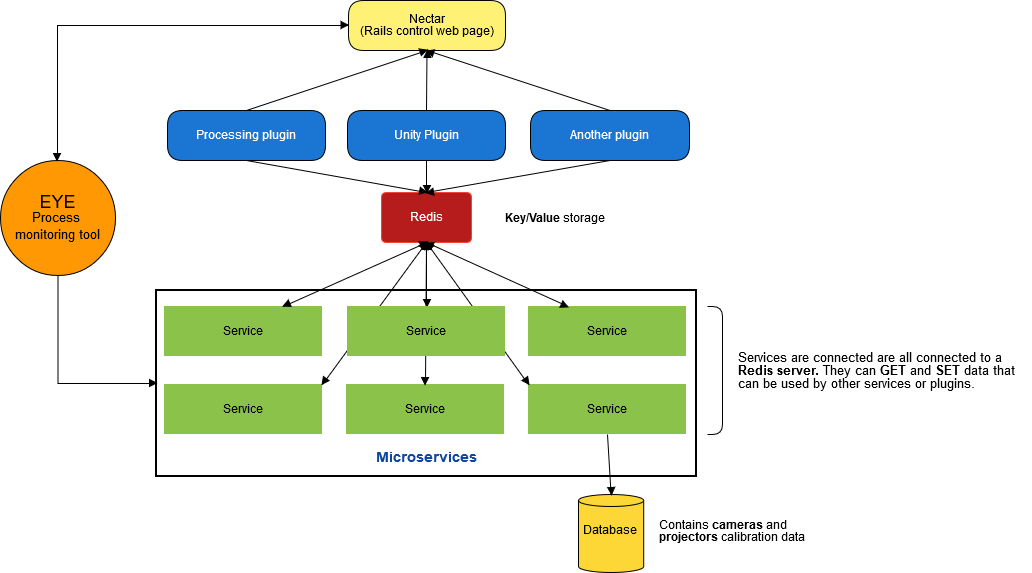
\includegraphics[width=\linewidth]{images/archi2}
\caption{Schéma de l'architecture en micro services développée}
\label{fig:microarchi}
\end{figure} 